%%% -*-LaTeX-*-

\chapter{A Complexity Spectrum for SweetPea designs}

The complexity of SweetPea designs greatly varies depending on the user's requirements. At one end of the spectrum are simple designs, in which there are no structured relationships between trials in a sequence. At the other end are the most complex designs, in which multiple structured relationships exist between multiple trials in a sequence at varying intervals. This chapter will present a precised gradation of 6 complexity tiers for experimental designs in order to facilitate future discussion. Recall that a complete experimental design is defined by a block, which is composed of a set of factors, a crossing of some subset of the factors, and a set of constraints. This section considers the complexity of a design based solely upon the factors present. Constraints on the overall design are not included in this gradation, as their complexity depends primarily on the complexity of the factors that they constrain.


\section{Factors and Windows}

\subsection{Factor Types}

Only two types of factors exist in SweetPea: \textit{Basic} and \textit{Derived}. The levels of a basic factor are literal values. Basic factors form the foundation of all designs. The following example declares a basic factor named \texttt{direction}, whose levels are the directions of the compass:

\begin{verbatim}
direction = Factor("Direction", ["North", "South", "East", "West"])
\end{verbatim}

On the other hand, the levels of a derived factor depend upon values from other factors in the design. The \texttt{congruency} characteristic in the Stroop experiment is expressed as a derived factor:

\begin{verbatim}
congruency = Factor("Congruency", [
  DerivedLevel("Congruent",   WithinTrial(lambda c, t: c == t, [color, text])),
  DerivedLevel("Incongruent", WithinTrial(lambda c, t: c != t, [color, text]))
])
\end{verbatim}

The level of the \texttt{congruency} factor is determined by the current levels of the \texttt{color} and \texttt{text} factors, which will vary for each trial in a generated sequence. \texttt{WithinTrial} denotes the \textit{window} of the derived level, which brings us to the next subject.

\subsection{Window Construction}

The construction of a derived level is based on the concept of a \textit{window}, which slices the trial sequence into segments which are considered to determine the current level of a derived factor. A window's dimensions are defined by a \textit{width} and \textit{stride}. The width indicates how many preceding trials, including the current trial, are to be considered. The \textit{stride} indicates how many trials to skip when moving on to the next trial for this factor.

The simplest type of window, for which \texttt{WithinTrial} is an alias, has a width and stride of one. This type of window does not span multiple trials. It only considers the values of basic factors within the same trial.

A slightly more complicated window has a width of two, but still a stride of one. (Aliased by the \texttt{Transition} window.) This type of window considers two adjacent trials for the purpose of inspecting the transition (or lack thereof) between them. For example, a \texttt{Transition} window would be appropriate when seeking to determine if a particular level was repeated in sequence.

\begin{verbatim}
direction_repeats = Factor("Direction Repetition", [
  DerivedLevel("Repeat",    Transition(lambda directions: directions[0] == directions[1], [direction])),
  DerivedLevel("No Repeat", Transition(lambda directions: directions[0] != directions[1], [direction]))
])
\end{verbatim}

The most complicated windows have arbitrary widths and strides. For example, a window with a width of one and a stride of four would consider the value of factors only at every fourth trial in the sequence. For example:

\begin{verbatim}
direction_is_north = Factor("Direction is North", [
  DerivedLevel("Direction is North",     Window(lambda direction: direction == "North", [direction], 1, 4)),
  DerivedLevel("Direction is not North", Window(lambda direction: direction != "North", [direction], 1, 4))
])
\end{verbatim}

Notice that windows with non-one width and stride will not have a value for every trial in the sequence. Generally speaking, a window with width $w$ and stride $s$ will first apply to trial $w$, and to every $s^{th}$ trial thereafter.

\begin{figure}[htb]
\centering
\centerline{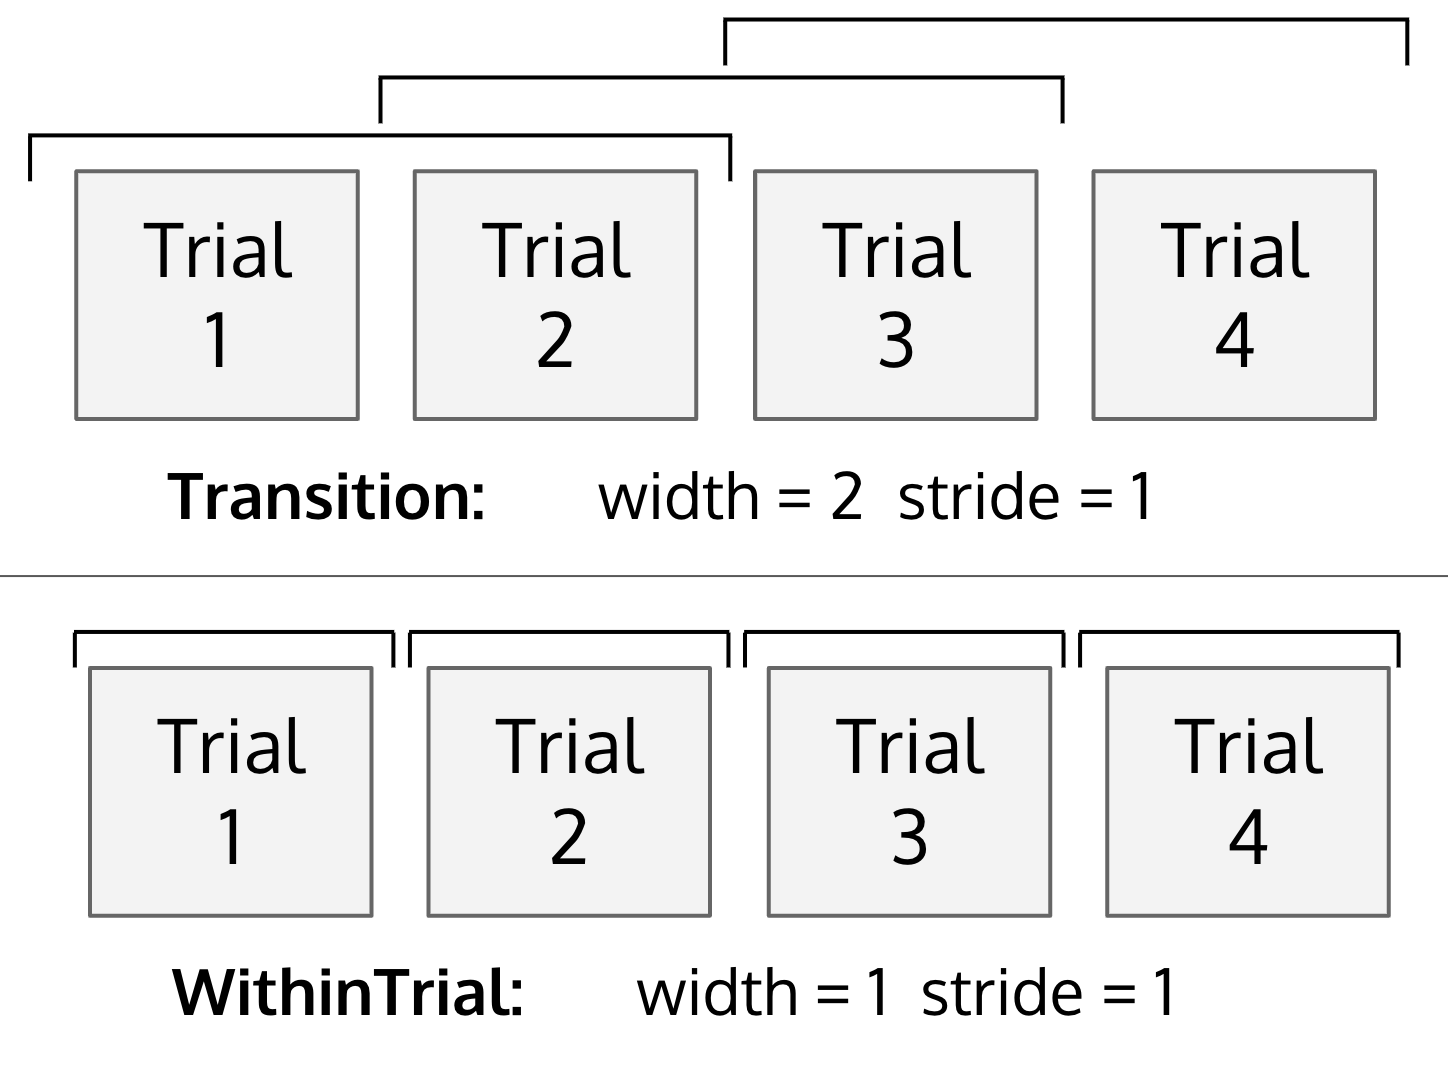
\includegraphics[origin=c,width=8cm]{../figures/windows.png}}
\caption{Window Properties}
\label{fig:windows}
\end{figure}


\section{Complexity Gradation}

Now understanding the types of factors and windows that can be used to define experimental designs, we can establish the complexity tiers with which to categorize different designs.

\subsection{Tier 1}

Tier 1 designs consist of basic factors only. No derived factors are allowed, and all factors in the design are crossed. Every valid trial sequence is a permutation of the crossed factors.

\begin{verbatim}
direction = Factor("Direction", ["North", "South", "East", "West"])
time_of_day = Factor("Time of Day", ["Sunrise", "High Noon", "Sunset"])
\end{verbatim}

\subsection{Tier 2}

Tier 2 designs still consist of only basic factors, but allow additional basic factors to be present which are uncrossed. Every valid trial sequence is a permutation of the crossed factors and random level selections for the uncrossed factors.

\subsection{Tier 3}

Tier 3 designs add derived factors with windows being limited to $width=1$ and $stride=1$. (\texttt{WithinTrial}) Every valid trial sequence is a permutation of the crossed factors and random level selections for the uncrossed basic factors. The values for uncrossed derived factors will depend upon the level selections of basic factors.

\begin{verbatim}
congruency = Factor("Congruency", [
  DerivedLevel("Congruent",   WithinTrial(op.eq, [color, text])),
  DerivedLevel("Incongruent", WithinTrial(op.ne, [color, text]))
])
\end{verbatim}

\subsection{Tier 4}

Tier 4 designs relax the window limits to $width=2$ and $stride=1$. (\texttt{Transition})

\begin{verbatim}
color_repeats = Factor("Color Repeats", [
  DerivedLevel("Repeat",    Transition(lambda c: c[0] == c[1], [color])),
  DerivedLevel("No Repeat", Transition(lambda c: c[0] != c[1], [color]))
])
\end{verbatim}


\subsection{Tier 5}

Tier 5 designs allow arbitrary values for the width and stride of all windows.

\begin{verbatim}
unconnected_color_repeats = Factor("Color Repeats (Unconnected)", [
  DerivedLevel("Repeat",    Window(lambda c: c[0] == c[1], [color], 2, 2)),
  DerivedLevel("No Repeat", Window(lambda c: c[0] != c[1], [color], 2, 2))
])
\end{verbatim}

